\section{Teori}
Teorin kommer att behandla fundamentala delar för arkitekturen och vilka olika möjligheter man har vid uppbyggnad av en arkitektur. Den beskriver även olika strategier man kan använda när man skapar arkitekturen och hur man ska få arkitekturen att uppnå de krav som finns.

\subsection{Arkitekturens grundpelare}
För att man ska kunna skapa en arkitektur så måste man från början ha en kravspecifikation, så man ska kunna veta vilka begränsningar man kommer ha på arkitekturen. Det kommer även vara dessa krav som man utgår ifrån när man ska designa arkitekturen.
\newline
\newline
Det kommer även krävas någon typ av kravdokumentation från kunden som beskriver hur kunden mer eller mindre vill att programmet ska se ut och hur det ska fungera. 
\newline
\newline
%Beroende på vad det är för typ av system som ska byggas så kan arkitekturen skapas på olika vis. T.ex.
Arkitekturen beror på vad det är för typ av system som ska byggas. Är det t.ex. ett väldigt litet system så är det inte alls säkert att det behövs en arkitektur, utan det kan vara möjligt att gå direkt från specifiktation till design av datastrukturer och algoritmer. Men är det istället ett väldigt stort system man ska bygga, så vill man gärna dela upp det i mindre moduler och komponenter, och det är just detta som arkitekturen gör. Så arkitekturen kan beskrivas som uppdelningen av ett system till flera mindre delar. \cite[s. 223]{set}
\newline
\newline
Mjukvaruarkitekturer kan också liknas mycket med byggnadsarkitekturer, de har en del saker gemensamt t.ex. 
\begin{enumerate}
	\item Flera vyer
	\item Arkitektoniska stilar
	\item Stil och ingenjörskonst
	\item Stil och material
\end{enumerate}
En byggnadesarkitekt arbetar med kunden i fråga om olika vyer när han vill betona en speciell del på byggnaden. Till exempel finns det förhöjningar och våningar som ger det yttre en ''top-down'' vy. \citep{perry92}

\subsection{Design och Arkitektur}
%Det finns många likheter mellan designen och arkitekturen, men det är viktigt att förstå skillnaden.
Vid designen av arkitekturen så är det bra om kravspecifikationen är skriven på ett sådant vis att det är funktion och inte form som är i fokus. När man ska bygga något är det bra om man har en design som beskriver mer hur komponenterna ska se ut och sedan arkitekturen som beskriver hur de hänger ihop. I det tidiga skedet är dock designen kopplad till arkitekturen, eftersom den beskriver hur arkitekturen ska se ut.
\newline
\newline
Skillnaden mellan design- och arkitekturbeslut, är att arkitekturen ska vara mer strukturell och systematisk för att man ska kunna uppnå kundens krav med hänsyn till t.ex. resurser. Eftersom arkitekturen även kommer vara grunden som man bygger systemet på, så kommer den vara svårast att ändra när man väl börjat. Det är dock inte omöjligt och inte ovanligt att ändra arkitekturen efterhand som nya problem eller förbättringar uppkommer eller om kunden skulle vilja ha någonting annorlunda. Den bästa arkitekturen är ändå den som efterhand går att förändra och anpassa efter nya förutsättningar.
\newline
\newline
Det svåra med designen av arkitekturen är att hålla koll på och tänka ut alla möjliga problem som skulle kunna uppstå i framtiden under utveckling och användning av systemet, t.ex. information som fattas eller är felaktig som systemet ska kunna hantera. Andra svårigheter som kan begränsa antalet möjligheter för arkitekturen är t.ex. icke funktionella krav, så som att systemet ska vara lätt att underhålla och vidareutveckla, att det ska vara lätt att använda och enkelt att porta till andra plattformar. Problemet med icke funktionella krav är att de inte enbart påverkar antalet möjligheter man har till arkitekturen, utan de kan även krocka med varandra. T.ex. så kan krav på att systemet ska vara stabilt och återanvändbart vara väldigt dyrt att genomföra och därmed krocka med krav på projektets budget. Det kan också vara andra faktorer som styr så som olika regler som måste följas, att hårdvaran man använder måste följa vissa specifikationer och att systemet ska fungera med äldre program. \cite[s. 224--225]{set}
\newline
\newline
Med detta taget i beaktning så finns det ingen specifik instruktion eller formel som man kan följa för att skapa en bra arkitektur. Det som krävs istället är kreativitet, att man är smart och tidigare erfarenheter, samt att man har tillgång till experterutlåtanden gällande olika val.
\newline
\newline
Ett bra sätt att träna på hur man ska göra smarta designbeslut är att man studerar redan existerande exempel på hur bra arkitekturer ser ut, och sedan återanvända lösningar från dessa till liknande problem. T.ex. så hittar erfarna utvecklare sällan på nya lösningar från grunden, utan lånar idéer från redan existerande lösningar och gör om dem för att de ska passa just deras design. Exempel på vad man kan ta in för källor för en bra design syns i figur \ref{fig:des}.
\newline
\newline
Det finns flera olika sätt som man kan använda andras lösningar på. Ett är t.ex. att man lånar hela designen inklusive koden och gör mindre förändringar för att det ska passa ens egna problem. Detta kan dock vara lite väl extremt och det finns risk att de strider mot upphovsrätt och annat, men det finns bättre lösningar för att göra ett liknande system med mindre variationer. Ett exempel är att göra designen utifrån en referensmodell, som är snarare en generell lösning för arkitekturen som beskriver hur systemet bör delas upp i de mindre delarna och hur dessa sedan interagerar med varandra. Sedan hur varje komponent ska se ut på detaljnivå och hur kommunikationen ska fungera mellan dem mer detaljerat beror mer på vad det är för typ av program och hur det ska fungera i praktiken. \cite[s. 226--227]{set}

\begin{figure}[h]
\centerline{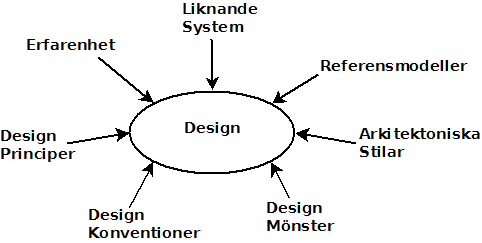
\includegraphics[scale=0.6]{sebastian-tex/grafik/designadvice.png}}
\caption{Källor till arkitekturdesignen.}
\label{fig:des}
\end{figure}

\paragraph{Processen}
Att ta fram en fungerande arkitektur är inget som blir klart direkt. Man måste gå fram och tillbaka och göra ändringar när man upptäcker nya problem eller möjligheter. Man vill kontrollera att det fortfarande är genomförbart, upptäcker man nya bättre lösningar kan man presentera dessa för kunden och se om man borde gå på den nya lösningen istället. Det som är allra viktigast är att hela tiden jämföra arkitekturen mot kravspecifikationen så man hela tiden uppfyller alla krav så att inget av dem blir omöjligt att genomföra. \cite[s. 228--230]{set} %Ett exempel på hur denna process går till syns i figur SIFFRA. HA EN FIGUR HÄR S. 229

\subsection{Arkitektoniska mönster}
Precis som det finns designmönster när man skriver kod, så finns det arkitektoniska mönster som beskriver hur man bör dela upp sitt system i mindre delar och hur de delarna ska interagera med varandra. Dessa fungerar inte direkt som referensmodeller som beskrevs i tidigare avsnitt, utan de beskriver mer generellt hur man bör möta olika designproblem istället för att fokusera på vissa typer av problem.
\newline
\newline
De arkitektoniska mönsterna är mycket bredare än designmönster och kan beskriva lösningar på flera olika problem inom mjukvaruutveckling, så som t.ex. begränsningar på hårdvara och hur man minimerar olika risker. De definieras också som att vara strikt beskrivande och för allmänheten tillgängliga.
\newline
\newline
Ibland kan det vara så att när man förbättrar en del av systemet så blir det motsatt effekt någon annanstans. Därför handlar det om att kunna välja ut flera olika arkitektoniska mönster som tillsammans kan hjälpa till att skapa en bra arkitekturdesign som på bästa sätt löser detta problem. \cite[s. 226--228]{set}

\subsection{Sammanfattning}
Det som går att sammanfatta teorin med är att det finns väldigt många olika sätt att göra arkitekturen på och det beror mycket på vad det är för typ av system som ska göras bl.a. om det är ett stort eller litet system påverkar utgången mycket. Kravspecifikationen är även väldigt viktig att arkitekturen uppfyller eftersom det är den som sätter kraven och målen för arkitekturen.
\newline
\newline
Vid utvecklandet av arkitekturen så är det väldigt bra om man kan ta inspiration från andra välskrivna arkitekturer och även använda sig av de olika arkitektoniska mönster som finns.
